\FloatBarrier

\begin{figure}[h!]
\centering
\caption{Full-Wave Bridge Rectifier Circuit}
\label{fig:fwr}
\begin{circuitikz}
	\draw
	( 0 , 4 ) to [ sV , v<=$20Vpp$ ] ( 0 , 0 )
	( 0 , 4 ) -- ( 4 , 4 ) to [ empty diode ] ( 6 , 2 )
	( 2 , 2 ) to [ empty diode ] ( 4 , 4 )
	( 2 , 2 ) to [ empty diode ] ( 4 , 0 )
	( 4 , 0 ) to [ empty diode ] ( 6 , 2 )
	( 4 , 0 ) -- ( 0 , 0 )
	( 2 , 2 ) to [ R = 300 <\ohm> ] ( 6 , 2 )
	( 2 , 2 ) node[label={ [font=\normalsize] above : $-$ } ] { }
	( 6 , 2 ) node[label={ [font=\normalsize] above : $+$ } ] { }
	;
\end{circuitikz}
\end{figure}

\FloatBarrier

Figure (\ref{fig:fwr}) displays a full-wave bridge rectifier circuit. The circuit's specification requires that it take an input sinusoidal signal and produce an output voltage that is the absolute value of that signal with the least amount of error possible. The output voltage is measured over the resistor, which shall be referred to as $R$. In reality, this ideal is not reached. The experiment demonstrates the degree to which the specification is satisfied.
The full-wave bridge rectifier circuit takes advantage of the fact that diodes essentially act as broken circuits when the applied voltage is less than its threshold voltage and act as short circuits when the applied voltage exceeds its threshold voltage. This is a simplification of the Shockley diode model:

\begin{equation}
	\label{eq:shockley_diode}
	I_{diode}( V_{applied} ) = I_0 ( e^{ \frac{qV_{applied}}{k_B T} } - 1 )
\end{equation}

In equation (\ref{eq:shockley_diode}), $I_0$ is the reverse saturation current, $q$ is the elementary charge, $k_B$ is Boltzmann's constant, and $T$ is temperature. A more ideal model treats the diode as the perfect switch described above, namely that the diode acts as a broken circuit unless $V_{applied}$ exceeds its threshold voltage, assumed to be about 0.7\si{\volt} and referred to as $V_{Th}$. Figure (\ref{fig:ideal_vs_shock}) below compares these two models in a graph. The graph demonstrates that this more idealized model accurately characterizes the behavior of the diode. It shall be used instead to describe the diode's characteristics.

\FloatBarrier

\begin{figure}[h!]
	\centering
	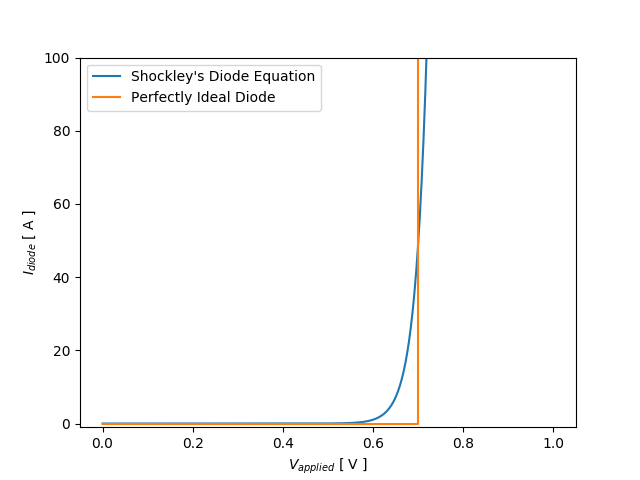
\includegraphics[scale=0.75]{../images/ideal_diode.PNG}
	\caption{Shockley Diode Model vs. Perfectly Ideal Diode}
	\label{fig:ideal_vs_shock}
\end{figure}

\FloatBarrier

{\footnotesize $I_0$ is set to 0.1\si{\nano\ampere}. Temperature is assumed to be 300\si{\kelvin}. Threshold voltage of perfectly ideal model is assumed to be 0.7\si{\volt}. }

\FloatBarrier

A diode is said to be enabled when the applied source voltage, which shall be called $V_{A}$, meets or exceeds its threshold voltage. Enabled diodes are drawn in green. Two cases are to be considered: when $V_{A} > 2V_{Th}$ and when $V_{A} < 2V_{Th}$. $2V_{Th}$ must be used since the voltage must enabled two diodes in series as seen in the figures below. Note that $|V_{A}| < 2V_{Th}$ is trivial since no voltage drops over the load resistor $R$.

When $V_{A} > 2V_{Th}$, the diodes in figure (\ref{fig:v_app_high}) are enabled. The voltage measured over the resistor is clearly positive due to the direction of positive current flow. The positive current flow direction is indicated by an arrow.

\FloatBarrier

\begin{figure}[h!]
\centering
\caption{Full-Wave Rectifier when $V_{A} > 2V_{Th}$}
\label{fig:v_app_high}
\begin{circuitikz}
	\draw
	( 0 , 4 ) to [ sV , v<=$20Vpp$ ] ( 0 , 0 )
	( 0 , 4 ) -- ( 4 , 4 ) to [ empty diode , color = green ] ( 6 , 2 )
	( 2 , 2 ) to [ empty diode ] ( 4 , 4 )
	( 2 , 2 ) to [ empty diode , color = green ] ( 4 , 0 )
	( 4 , 0 ) to [ empty diode ] ( 6 , 2 )
	( 4 , 0 ) -- ( 0 , 0 )
	( 2 , 2 ) to [ R = 300 <\ohm> , i<_=$I$ ] ( 6 , 2 )
	( 2 , 2 ) node[label={ [font=\normalsize] above : $-$ } ] { }
	( 6 , 2 ) node[label={ [font=\normalsize] above : $+$ } ] { }
	;
\end{circuitikz}
\end{figure}

\FloatBarrier

Figure (\ref{fig:v_app_low}) demonstrates the case when $V_{A} < 2V_{Th}$. Again, the output voltage taken over the resistor is positive due to the direction of positive current flow.

\FloatBarrier

\begin{figure}[h!]
\centering
\caption{Full-Wave Rectifier when $V_{A} < 2V_{Th}$}
\label{fig:v_app_low}
\begin{circuitikz}
	\draw
	( 0 , 4 ) to [ sV , v<=$20Vpp$ ] ( 0 , 0 )
	( 0 , 4 ) -- ( 4 , 4 ) to [ empty diode ] ( 6 , 2 )
	( 2 , 2 ) to [ empty diode , color = green ] ( 4 , 4 )
	( 2 , 2 ) to [ empty diode ] ( 4 , 0 )
	( 4 , 0 ) to [ empty diode , color = green ] ( 6 , 2 )
	( 4 , 0 ) -- ( 0 , 0 )
	( 2 , 2 ) to [ R = 300 <\ohm> , i<_=$I$ ] ( 6 , 2 )
	( 2 , 2 ) node[label={ [font=\normalsize] above : $-$ } ] { }
	( 6 , 2 ) node[label={ [font=\normalsize] above : $+$ } ] { }
	;
\end{circuitikz}
\end{figure}

\FloatBarrier

A more quantitative description of this behavior can be obtained. In the $V_{A} > 2V_{Th}$ case, Kirchhoff's voltage law may be applied:

\FloatBarrier

\begin{figure}[h!]
\centering
\caption{Kirchhoff's Voltage Law for $V_{A} > 2V_{Th}$}
\label{fig:kvl_app_high}
\begin{circuitikz}
	\draw
	( 0 , 4 ) to [ sV , v<=$20Vpp$ ] ( 0 , 0 )
	( 0 , 4 ) -- ( 4 , 4 ) to [ empty diode , color = green ] ( 6 , 2 )
	( 2 , 2 ) to [ empty diode , color = green ] ( 4 , 0 )
	( 4 , 0 ) -- ( 0 , 0 )
	( 2 , 2 ) to [ R = 300 <\ohm> , i<_=$I$ ] ( 6 , 2 )
	( 2 , 2 ) node[label={ [font=\normalsize] above : $-$ } ] { }
	( 6 , 2 ) node[label={ [font=\normalsize] above : $+$ } ] { }
	( 1.5 , 1 ) node[scale=3]{$\circlearrowright$}
	;
\end{circuitikz}
\end{figure}

\FloatBarrier

\begin{equation}
	\label{eq:kvl_va_gt_2vth}
	+V_{A} - V_{Th} - V_{out} - V_{Th} = 0 \rightarrow V_{out} = V_{A} - 2V_{Th}
\end{equation}

The same method can be applied to the $V_{A} < 2V_{Th}$ case.

\FloatBarrier

\begin{figure}[h!]
\centering
\caption{Kirchhoff's Voltage Law for $V_{A} > 2V_{Th}$}
\label{fig:kvl_app_low}
\begin{circuitikz}
	\draw
	( 0 , 4 ) to [ sV , v<=$20Vpp$ ] ( 0 , 0 )
	( 0 , 4 ) -- ( 4 , 4 )
	( 2 , 2 ) to [ empty diode , color = green ] ( 4 , 4 )
	( 4 , 0 ) to [ empty diode , color = green ] ( 6 , 2 )
	( 4 , 0 ) -- ( 0 , 0 )
	( 2 , 2 ) to [ R = 300 <\ohm> , i<_=$I$ ] ( 6 , 2 )
	( 2 , 2 ) node[label={ [font=\normalsize] above : $-$ } ] { }
	( 6 , 2 ) node[label={ [font=\normalsize] above : $+$ } ] { }
	( 1.5 , 1 ) node[scale=3]{$\circlearrowright$}
	;
\end{circuitikz}
\end{figure}

\FloatBarrier

\begin{equation}
	\label{eq:kvl_va_lt_2vth}
	+V_{A} + V_{Th} + V_{out} + V_{Th} = 0 \rightarrow V_{out} = - V_{A} - 2V_{Th}
\end{equation}

These behaviors can be generalized in the following result for the output voltage of the full-wave rectifier circuit in figure (\ref{fig:fwr}):

\begin{equation}
	\label{eq:fwr_eq}
	V_{out}(V_{A}) = max( |V_{A}| - 2V_{Th} , 0 )
%	\begin{cases}
%		|V_{A}| - 2V_{Th} , & |V_{A}| > 2V_{Th} \\
%		0 , & \text{otherwise}
%	\end{cases}
\end{equation}

A plot of the expected output voltage against the input voltage is shown in figure (\ref{fig:expected_out_vs_in_fwr}):

\FloatBarrier

\begin{figure}[h!]
	\centering
	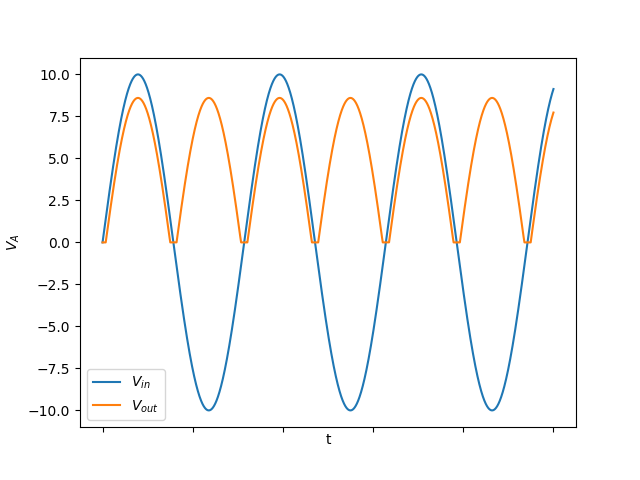
\includegraphics[scale=0.75]{../images/full_wave_rect.PNG}
	\caption{Full-Wave Bridge Rectifier Expected Result}
	\label{fig:expected_out_vs_in_fwr}
\end{figure}

\FloatBarrier

The measured result is presented in figure (\ref{fig:measured_fwr}) below:

\FloatBarrier

\begin{figure}[h!]
	\centering
	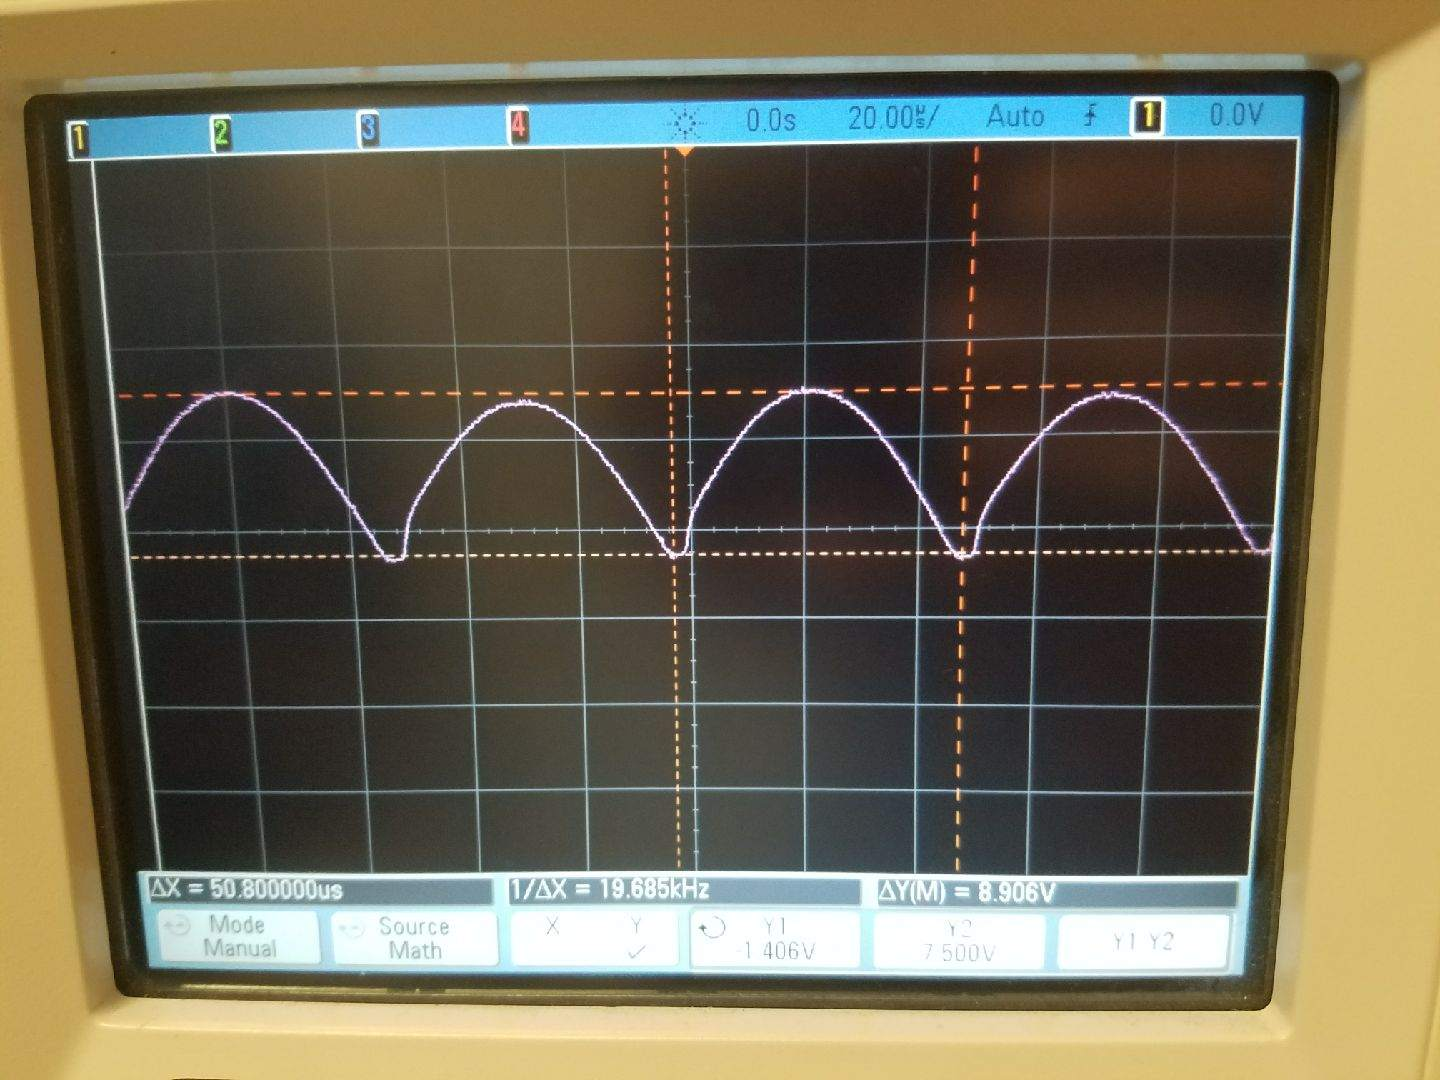
\includegraphics[scale=0.25]{../images/full_wave_rect_measured_amp.PNG}
	\caption{Measured Amplitude of Full-Wave Rectifier}
	\label{fig:measured_fwr}
\end{figure}

\FloatBarrier

The oscilloscope cannot directly measure the output voltage because the probe must be connected to ground. Thus, in figure (\ref{fig:measurement_scheme}), $V_1$ and $V_0$ are probed:

\FloatBarrier

\begin{figure}[h!]
\centering
\caption{Full-Wave Bridge Rectifier Circuit}
\label{fig:fwr}
\begin{circuitikz}
	\draw
	( 0 , 4 ) to [ sV , v<=$20Vpp$ ] ( 0 , 0 )
	( 0 , 4 ) -- ( 4 , 4 ) to [ empty diode ] ( 6 , 2 )
	( 2 , 2 ) to [ empty diode ] ( 4 , 4 )
	( 2 , 2 ) to [ empty diode ] ( 4 , 0 )
	( 4 , 0 ) to [ empty diode ] ( 6 , 2 )
	( 4 , 0 ) -- ( 0 , 0 )
	( 2 , 2 ) to [ R = 300 <\ohm> ] ( 6 , 2 )
	( 2 , 2 ) node[label={ [font=\normalsize] above : $V_0$ } ] { }
	( 6 , 2 ) node[label={ [font=\normalsize] above : $V_1$ } ] { }
	;
\end{circuitikz}
\end{figure}

\FloatBarrier

Without proof, $V_{out} = V_1 - V_0$. Thus, by subtracting these voltages, $V_{out}$ can be measured. $V_{out}$ is displayed with $V_1$ in yellow and $V_0$ in green in figure (\ref{fig:measured_fwr_with_inputs}) below:

\FloatBarrier

\begin{figure}[h!]
	\centering
	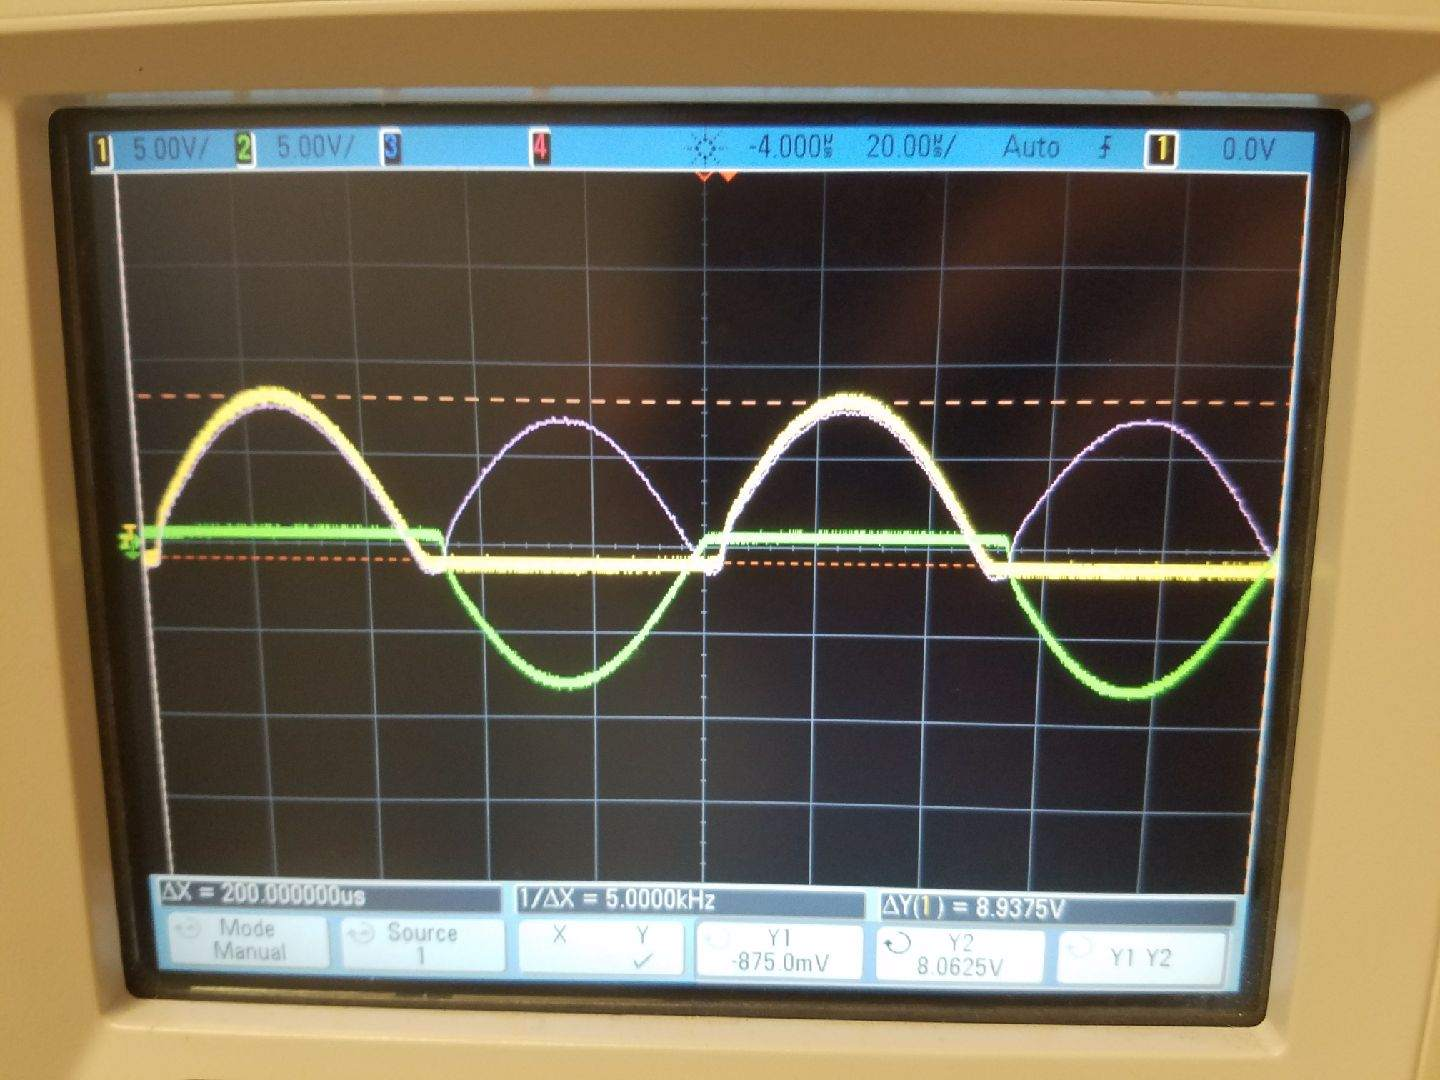
\includegraphics[scale=0.25]{../images/full_wave_rectifier.PNG}
	\caption{Measured Amplitude of Full-Wave Rectifier with Input Signals}
	\label{fig:measured_fwr_with_inputs}
\end{figure}

\FloatBarrier

{\footnotesize Input voltage is 20\si{\volt}pp. Frequency is 10\si{\kilo\hertz}.}

\FloatBarrier

The input source voltage could not be captured in the same plot. This is because only two probes for the oscilloscope are available. Two are required to measure the output voltage in this manner. Thus, a third would be needed to measure the input signal. \\

The peak and trough voltages of $V_{out}$ relative to the input supply voltage $V_{A}$ (as determined from the reading on the power supply) are reported in table (\ref{tab:peak_n_trough}). Note that the absolute value of all voltages is reported:

\FloatBarrier

\begin{table}[h!]
	\centering
	\caption{Peak and Trough Voltages of $V_{out}$ and $V_{A}$}
	\label{tab:peak_n_trough}
	\csvautotabular{../tables/fwr_data.csv}
\end{table}

\FloatBarrier

Equation (\ref{eq:fwr_eq}) predicts that the absolute value of the peak of $V_{out}$ is below the absolute value of the peak or trough of $V_{A}$ by $2V_{Th}$, assuming that $|V_{A}|$ at the peak and trough meets or exceeds $2V_{Th}$. Table (\ref{tab:theory_vs_practice}) presents the results compared to theory. The full-wave bridge rectifier very closely aligns with theoretical results:

\FloatBarrier

\begin{table}[h!]
	\centering
	\caption{Theoretical vs. Measured Results for Full-Wave Rectifier}
	\label{tab:theory_vs_practice}
	\csvautotabular{../tables/fwr_err.csv}
\end{table}

\FloatBarrier
